\documentclass[11pt,twoside,openright]{mpreport}
\usepackage[utf8]{inputenc}
\usepackage[T1]{fontenc}
\usepackage{textcomp}
\usepackage{mathptmx}
\usepackage[scaled=0.85]{helvet}
\usepackage{hyperref}
\usepackage{ngerman}
\usepackage[toc]{glossaries}
\usepackage{listings}
\usepackage{url}



\makeindex

% makeglossaries bericht.glo

\newacronym{rup}{RUP}{Rational Unified Prozess}
\newacronym{ide}{IDE}{Integrated Development Environment}

\newacronym{api}{API}{Application Programming Interface}
\newacronym{orm}{ORM}{Object-relational mapping}

\newglossaryentry{sqlite}{
	name=SQLite,
	description={SQLite ist eine Cross Plattform Datenbankengine, welche ohne Konfiguration auskommt. Es handelt sich dabei um eine Datenbank in einer Datei},
	first={SQLite}
}

\newglossaryentry{json}{
	name={JSON},
	description={JavaScript Object Notation (JSON), ist eine Notation zur Darstellung von Objekten in Textform},
	first={JavaScript Object Notation (JSON)}
}

\newglossaryentry{enum}{
	name={Enum},
	description={Ein Enum ist ein Datentyp mit fest bestimmten Konstanten. Es kann immer nur ein Wert ausgewählt sein.}
}

\newglossaryentry{splashscreen}{
	name={Splashscreen},
	description={Eine Anzeige, die oftmals beim Start einer Applikation die Wartezeit bis zur vollständigen Initialisierung überbrückt.}
}
\newglossaryentry{csv}{
	name={CSV},
	description={Ein Dateiformat, bei welchem die Datensätze über ein Trennzeichen voneinander getrennt sind.},
	first={Comma Separated Values (CSV)}
}
\newglossaryentry{http}{
	name={HTTP},
	description={Das Hypertext Transfer Protocol (HTTP) ist ein weit verbreitetes Protokoll, um Daten und Inhalte im Web zu übertragen. In dieser Arbeit wird es in der Kommunikation mit dem Server verwendet.},
	first={Hypertext Transfer Protocol (HTTP)}
}
\newglossaryentry{junit}{
	name={JUnit Test},
	description={Java bietet die Möglichkeit integrierte Softwaretests automatisiert durchzuführen. Dies erleichtert die Arbeit enorm und unterstützt ein Entwicklungsteam, eine möglichst hohe Testabdeckung zu erarbeiten},
	first={Java Unit Test (JUnit)}
}

\newglossaryentry{chronofunk}{
	name={Chronofunk},
	description={Die Motorradfahrer, welche im Rennfeld verteilt mitfahren und die Positionen der Ausreissergruppen per Funk an den RadioTour Speaker übermitteln}
}

\makeglossaries

\begin{document}

\setlength{\oddsidemargin}{50mm}
	\title{Android Applikation RadioTour}
	\author{Florian Bentele \& Daniel Stucki}
 	\maketitle

\chapter*{Abstract}


Bisher mussten bei Radrennen Motorradfahrer die Nummern der Fahrer, welche aus dem Feld ausgerissen sind, einem \textit{RadioTour Speaker} melden. Dieser meldet dann die Ausreisser jeweils per Funk an die Mannschaftsleiter weiter. Bei den meisten Radrennen notieren die \textit{RadioTour Speaker} die erhaltenen Informationen auf einem Notizbuch, bevor sie die Fahrernummern weitergeben. An der Tour de Suisse arbeitet man seit einigen Jahren mit einer Tablet-PC Web Applikation zur elektronischen Erfassung der Renninformationen.
\\
Die im Rahmen dieser Studienarbeit realisierte \textit{RadioTour} Android Tablet Applikation ersetzt und erweitert die "`in die Jahre gekommene"' webbasierte Tablet-PC Anwendung. Die neue native \textit{RadioTour} Android Anwendung bietet eine einfachere Touchscreen Bedienung, verbesserte Importfunktionen sowie neue Features wie beispielsweise Live-Marschtabellen und Streckenkilometerbestimmung aus den lokalen GPS-Daten. Verbessert wurde auch die Kommunikation mit der TourLive Webseite via JSON zur unmittelbaren Veröffentlichung der aktuellen Rennsituationen. Die Anwendung ist bewusst für Android Honeycomb \& Ice Cream Sandwich und für die  spezifische Hardware-Plattform eines Samsung Galaxy Tab 10.1 entwickelt worden, da das System zusammen mit der Hardware-Plattform zur Verfügung gestellt wird.
\\
Für die Entwicklung der Applikation kommt die Java IDE Eclipse (Version Indigo) zur Anwendung. Die Datenpersistierung auf dem Tablet wird mithilfe der ORMLite Library (Version 4.39) in einer SQLite Datenbank umgesetzt.
\\
Der Release 1 wurde an der Berner Rundfahrt 2012 getestet. Die dort gewonnenen Erkenntnisse wurden im Release 2 berücksichtigt, so dass nun ein System vorliegt, welches die Grundanforderungen erfüllt. Letzte, kleinere Anpassungen wird der Industriepartner im Rahmen der Systemübernahme vornehmen. Die neue RadioTour Anwendung wird voraussichtlich bei der Tour de Suisse 2012 zum Einsatz kommen.


\tableofcontents

\chapter*{Aufgabenstellung}

\begin{tabular}{ll}
Studiengang: & Informatik (I)\\
Semester: & FS 2012 (21.02.2012-01.06.2012)\\
Institut: & ITA: Internet-Technologien und Anwendungen\\
Gruppe: & Florian Bentele, Daniel Stucki\\
Verantwortlicher: & Dr. Prof. Peter Heinzmann, pheinzma@hsr.ch\\
Industriepartner: & cnlab AG, Lukas Frey, lukas.frey@cnlab.ch

\end{tabular}

\section*{Ausgangslage}
Bei Radrennen erfasst der so genannte \textit{RadioTour Speaker} Informationen zur Rennsituation, welche ihm von Motorradfahrern per Funk geliefert werden. Gegenwärtig legt der \textit{RadioTour Speaker} mit Hilfe einer TabletPC Web-Anwendung per Click auf die erhaltenen Fahrernummern die Zusammensetzung der Gruppen fest. Er tippt auch die Zeitabstände zwischen den Gruppen ein. Die \textit{RadioTour} Anwendung  visualisiert die Fahrergruppen und liefert Detailinformationen zu den Fahrern (z.B. Namen, Team, virtueller Rang). Veränderungen in den Fahrergruppen können per Drag-and-Drop nachgeführt werden. Die mit der \textit{RadioTour} Anwendung erfassten Rennsituationen werden per Mobilfunknetz zu einem Webserver gesendet, wo sie weiteren Anwendungen, z.B. Live Webinformationen zur Verfügung stehen.

\section*{Ziel}
Die aus dem Jahre 2006 stammende Notebook Web Applikation soll nun dahingehend überarbeitet und erweitert werden, dass man sie auf Android-Tablets oder iPads betreiben kann.
\\
Das Produkt wird spezifisch auf ein Gerät und nicht plattformübergreifend entwickelt. Die Verbindung zum Server wird in der Arbeit definiert, jedoch werden keine serverseitigen Entwicklungen erarbeitet.
\\
Die Mehrsprachigkeit wird nach Android Standards implementiert \footnote{Android Internationalisierung, \url{http://developer.android.com/guide/topics/resources/localization.html}}. Eine Übersetzung ist jedoch nicht Teil der Arbeit.
\newpage

\section*{Teilaufgaben}
\begin{itemize}
\item Analyse der existierenden \textit{RadioTour} und TourLive-Anwendungen
\begin{itemize}
\item Tour de Suisse Dokumente
\item Alte \textit{RadioTour} Anwendung\\
\url{http://gps.cnlab.ch/tablet/}\\
user: ba\_tourlive\\
password: access4tl
\item TourLive-System (GPS Positions- und Bilderfassungssysteme, Webanwendung)
\item Kommunikation \textit{RadioTour} – TourLive-Webanwendung
\item Vergleich mit Systemen anderer Radrennen 
\end{itemize}

\item Festlegung der Funktionalität der neuen Tablet-Anwendung (Requirements Engineering)
\begin{itemize}
\item Studium der Geschäftsprozesse (Renninformationen, Rennverlauf)
\item Austesten von Teilfunktionen (Android-Tablet Programmierung, GPS-Positionserfassung, Usability Experimente)
\item Erweiterte Funktionen (z.B. Erfassung der Streckenkilometer, Integration von Marschtabellen)
\item Auswahl der Hardware-Plattform
\item Spezifikation
\end{itemize}

\item Design
\begin{itemize}
\item Benutzerschnittstelle
\item Kommunikation mit TourLive Aufnahmesystemen (Weitergabe der Daten an Datenserver)
\item \textit{RadioTour} Anwendung
\end{itemize}

\item Realisierung
\begin{itemize}
\item Prototypen
\item Anpassungen
\item Friendly User Test Version (Beta-Release)
\item Feldtest an einem Radrennen
\item Übergabe an cnlab
\end{itemize}

\item Dokumentation
\begin{itemize}
\item Gemäss Anforderungen Industriepartner (das System soll vom Industriepartner betrieben und erweitert werden können)
\item Bericht gemäss HSR / Heinzmann Richtlinien
\end{itemize}
\end{itemize}

Diese Aufgabenstellung wird genehmigt vom Betreuer
\\
\\

\begin{tabular}{p{3cm}p{4cm}}
\hline
Ort / Datum & P. Heinzmann
\end{tabular}

\section*{Erklärung zur Urheberschaft\footnote{Diese Erklärung basiert auf der Muster-Erklärung in den Richtlinien der HSR zur Durchführung von Projekt-, Studien-, Diplom- oder Bachelorarbeiten vom 16. Februar 2009.}}
Die vorliegende Arbeit basiert auf Ideen, Arbeitsleistungen, Hilfestellungen und Beiträgen gemäss folgender Aufstellung:
\\

\begin{tabular}{|m{5cm}|m{3.7cm}|m{3cm}|}
\hline
Gegenstand, Leistung & Person & Funktion \\[5pt]\hline\hline
Kapitel 3, 4, 5 und Anhänge & Daniel Stucki & Autor der Arbeit\\[5pt]\hline
Kapitel 1, 2, 5, 6 und Anhänge & Florian Bentele & Autor der Arbeit\\[5pt]\hline
Korrektur & Heinrich Stucki & Lektorat \\[5pt]\hline
Korrektur & Doris Bentele & Lektorat \\[5pt]\hline
Korrektur & Ursina Bentele & Lektorat \\[5pt]\hline
Idee, Aufgabenstellung, allgemeines Pflichtenheft, Betreuung während der Arbeit & Prof. Dr. P. Heinzmann & Verantwortlicher Professor \\[5pt]\hline
Industriepartner und Ansprechperson & Lukas Frey & cnlab AG \\[5pt]\hline
\end{tabular}
\\
\\

Ich erkläre hiermit,
\begin{itemize}
\item dass ich die vorliegende Arbeit gemäss obiger Zusammenstellung selber und ohne weitere fremde Hilfe durchgeführt habe,
\item dass ich sämtliche verwendeten Quellen erwähnt und gemäss gängigen wissenschaftlichen Zitierregeln korrekt angegeben habe.
\end{itemize}

Rapperswil, 29. Mai 2012
\\
\\

\begin{tabular}{p{5cm}p{5cm}}
\hline

Florian Bentele & Daniel Stucki
\end{tabular}

\newpage

\section*{Vereinbarung zur Verwendung und Weiterentwicklung der Arbeit\footnote{Diese Vereinbarung basiert auf den Muster-Vereinbarungen in den Richtlinien der HSR zur Durchführung von Projekt-, Studien-, Diplom- oder Bachelorarbeiten vom 16. Februar 2009.}}

\textbf{1. Gegenstand der Vereinbarung}
\\
Mit dieser Vereinbarung werden die Rechte über die Verwendung und die Weiterentwicklung der Ergebnisse der \thesistype \ "`\thesistitle "'  von \thesisauthora \ und \thesisauthorb \ unter der Betreuung von \professor \ (für die Arbeit verantwortlicher Professor) geregelt.
\\

\textbf{2. Urheberrecht}
\\
Die Urheberrechte stehen der Studentin / dem Student zu.
\\

\textbf{3. Verwendung}
\\
Die Ergebnisse der Arbeit dürfen sowohl von allen an der Arbeit beteiligten Parteien, d.h. von den Studenten, welche die Arbeit verfasst haben, vom verantwortlichen Professor sowie vom Industriepartner verwendet und weiter entwickelt werden. Die Namensnennung der beteiligten Parteien ist bei der Weiterverwendung erwünscht, aber nicht Pflicht.
\\

\begin{tabular}{p{5cm}p{1cm}p{6cm}}
Rapperswil, den  & & \\[30pt]
\hline
 & & \thesisauthora \\[10pt]
Rapperswil, den  & & \\[30pt]
\hline
 & & \thesisauthorb \\[10pt]
Rapperswil, den  & & \\[30pt]
\hline
 & & \professor \\[10pt]
Rapperswil, den  & & \\[30pt]
\hline
 & & Industriepartner, Lukas Frey, cnlab AG \\
\end{tabular}

\chapter*{Management Summary}

\section*{Ausgangslage}
An der Tour de Suisse fahren ca. 200 Radrennfahrer in Tagesetappen durch die ganze Schweiz. Dabei werden Sie von diversen Motorfahrzeugen begleitet. Im Radfahrer-Feld fährt ebenfalls der \textit{RadioTour Speaker} mit. Seine Funktion besteht darin, Live Informationen des Rennens zu erfassen und an den Server der cnlab AG weiterzuleiten.  Die Übertragung der Daten vom Gerät zum Server geschieht über das Mobilfunknetz 3G.

\subsection*{Live Informationen}
Während dem Rennen werden aus verschiedenen Quellen Informationen gesammelt. Zum einen sind dies Veränderungen im Rennfeld, zum anderen Wertungen, welche die Fahrer erreichen können, so z.B. einen Bergsprint. Diese Daten werden vom \textit{RadioTour Speaker} manuell erfasst.
\\
Wenn sich ein Rennfahrer vom Feld ablöst und einen Vorsprung erarbeitet, wird dieser von einem Motorradfahrer verfolgt. Diese Änderung wird dann sofort per Funk an den \textit{RadioTour Speaker} übermittelt.

\subsection*{Äussere Bedingungen}
Bei Live Sport Events wie der Tour de Suisse ist die Erfassung von Echtzeitdaten, aus technischer Sicht, eine Herausforderung. Sowohl das Alpine Gebirge, wo die Mobilfunkverbindungen und GPS Informationen nicht immer gewährleistet sind, als auch die ständige Vibration der Fahrzeuge stellen erschwerende Rahmenbedingungen dar.
\\
Die Unterbrüche der Verbindung werden überbrückt, indem die Änderungen gesammelt und periodisch an den Server gesendet werde. Alle Änderungen werden als Paket in eine Warteschlange eingetragen. Ist eine sofortige Übertragen nicht möglich, wird es später wieder versucht.


\section*{Vorgehensweise}
In der vorliegenden Studienarbeit kommt das Vorgehensmodell zur Softwareentwicklung von \gls{rup} zur Anwendung. Das Projekt wird in die folgenden vier Phasen aufgeteilt:

\begin{enumerate}
\item Inception
\item Elaboration
\item Construction
\item Transition
\end{enumerate}

In jeder dieser Phasen werden die Arbeitsschritte nach \gls{rup} durchgeführt, je nach dem in mehreren Iterationen, wie es bei dieser Arbeit in der Phase \textit{Construction} vorkommt.\footnote{Wikipedia, Rational Unified Process,  \url{http://de.wikipedia.org/wiki/Rational_Unified_Proces}, aufgerufen am 20.05.2012.}
\\
Die Erfassung der Anforderungen, der Entscheid zur Entwicklung auf einem Android Gerät sowie die Evaluation eines geeigneten Tablets bilden zusammen die Startphase des Projekts. Die Anforderungskriterien an das Tablet wurden in einer Sitzung zusammen mit Herrn Dr. Prof. Peter Heinzmann, dem Betreuer der Arbeit, diskutiert und genehmigt.
\\
Im weiteren Verlauf der Arbeit wurden die Anforderungen und die UseCases definiert. Daraus entstand dann die Domainlogik und parallel dazu ein erster Prototyp des UserInterface. Insbesondere die Benutzerschnittstelle entstand in mehreren Iterationen, da eine gute Bedienung für den Erfolg des Produktes entscheidend ist, dies jedoch erst bei der realen Anwendung geprüft werden kann.

\section*{Ergebnisse}
Die \textit{RadioTour} Android Applikation beinhaltet die festgelegten Anforderungen. Die Fahrerlisten und die offiziellen Zeitmessungen können via USB oder aus dem Internet importiert werden. Die Gruppen lassen sich dynamisch verändern und die Rennsituation wird an den Server übermittelt. Ein Testlauf mit dem ersten Prototypen hat klar aufgezeigt, dass diese Anwendung eine Verbesserung in der Bedienung bringt. Dabei entstehen keine Einbussen in der Funktionalität. Die Applikation ist damit für den Einsatz an der Tour de Suisse bereit.


\section*{Ausblick}
Für den erfolgreichen Einsatz an der Tour de Suisse ist ein Feldtest, insbesondere um die Serververbindung zu testen, notwendig.
\\
Nach der Tour de Suisse sind die Eindrücke und das Feedback des \textit{RadioTour Speakers} aufzunehmen, damit die Applikation weiter verbessert werden kann.

\chapter{Einleitung}

Im folgenden Abschnitt werden die aus technischer Sicht relevanten Aspekte genauer analysiert. Zu Beginn wird das Aufgabenumfeld in einem weiteren Sinne betrachtet, später gehen wir konkret auf die Analyse und das Software Engineering ein.
\\

Der Hauptteil richtet sich vor allem an Personen, die bereits Hintergrundwissen zum Betriebssystem Android vorweisen sowie für Entwickler, die an der Weiterentwicklung des Produktes interessiert sind.

\section{BigPicture}
Zur Übersicht wird das Umfeld der Applikation in einem BigPicture zusammengefasst. Es ermöglicht die Darstellung der äusseren Einflussfaktoren sowie die Abgrenzung des Systems zu definieren.

\begin{figure}[h!]
\caption{BigPicture}
\centering
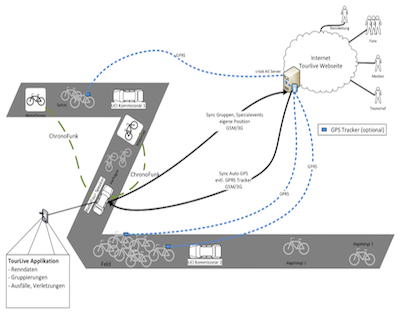
\includegraphics{05technischerbericht/images/big_picture.png}
\end{figure} 

Die schematische Darstellung zeigt im wesentlichen die drei Hauptaktoren auf. Zum einen sind dies die Motorradfahrer, welche die Radrennfahrer begleiten und Veränderungen in Echtzeit per Funk übermitteln. Diese Informationen kommen in kurzen Abständen und müssen sofort erfasst werden können. Im UserInterface verwenden wir dafür eine Lösung bei der mehrere Radrennfahrer gleichzeitig eingetragen werden können.
\\

Eine weitere Rolle spielt der \textit{RadioTour Speaker} mit dem Android Tablet. Er fasst die Informationen zusammen und wertet diese bereits auf dem Gerät aus. Im Tablett werden auch Daten wie z.B. die Durchschnittsgeschwindigkeit und die aktuelle Rennzeit angezeigt.
\\
Der dritte Aktor bildet der Server der \textit{cnlab AG}, welcher direkt mit der Applikation kommuniziert. Ausgetauscht werden die Veränderungen im Feld sowie markante Rückstände von der Spitze. Weiter können Ereignisse wie z.B. eine Verletzung oder ein defektes Fahrrad aufgezeichnet werden. Die Daten werden dann weiter auf der Webseite der \textit{TourLive} aufbereitet und publiziert. Nicht nur für die beteiligten im Team sondern auch für Fans sind diese Angaben von grossem Interesse, da die Daten vor den offiziellen Zeitmessungen bereits einen Einblick in das Schlussklassement geben.

\section{Evaluation und Kaufempfehlung}
Die Evaluation der Zielplattform war ein wichtiger Faktor für die weitere Entwicklung der Arbeit. Aus diesem Grund stand dies ganz zu Beginn der Arbeit an. Zur Auswahl standen die beiden marktführenden Betriebssysteme Android und iOS. Als Grundlage für die Evaluation dienten die folgenden Kriterien:
\begin{itemize}
\item Vorkenntnisse der Programmiersprachen Java bzw. Objective-C
\item Möglichkeiten zum UserInterface Design
\item Programmierumgebung, \gls{ide}
\item mögliche Vertriebskanäle der Applikation
\item Nutzbarkeit von externen Geräten und Schnittstellen
\item Vielfalt von Informationsquellen im Internet
\end{itemize}
Die Kriterien werden in einer Nutzwertanalyse gewichtet und bewertet. Insbesondere die Vorkenntnisse in Java sind  ausschlaggebend für den Entscheid, die Applikation für die Androidplattform zu entwickeln. Dieser Entscheid ist in Absprache mit Herrn Heinzmann getroffen worden. Die gesamte Liste der Kriterien mit der jeweiligen Gewichtung sowie eine ausführliche Erläuterung befinden sich im Anhang \ref{ref_kriterien}.
\\

Für die Auswahl eines geeigneten Tablets wird im nächsten Schritt ein Kriterienkatalog definiert mit zwingenden und optionalen Kriterien für das Gerät. Die zwingenden Kriterien beinhalten:
\begin{itemize}
\item Android Betriebssystem, gemäss Evaluation
\item USB Anschluss für den Import der Fahrerliste am Renntag, optional auch mit Adapter möglich
\item Mobilfunktnetz 3G für die Kommunikation mit dem Server
\item GPS für die Lokalisierung
\item Stromversorgung durch 12V (Auto) Adapter möglich
\end{itemize}
Zu den optionalen Kriterien gehören die Akkulaufzeit, falls die Stromversorgung unterbrochen wird sowie ein grosszügiger Bildschirm für die Bedienung mit dem Finger oder mithilfe eines Stiftes.
\\

Als Sieger und somit auch als Kaufempfehlung an die \textit{cnlab AG} geht das Lenovo ThinkPad Tablet. Dieses Gerät erfüllt alle Kriterien und überzeugt in der Vielfalt der Anschlüsse. Die Kaufempfehlung mit weiteren Erläuterungen ist ebenfalls im Anhang \ref{ref_kaufempfehlung} zu finden.
\\

Im Verlauf der Arbeit ist ein defekt an der Micro USB Buchse entstanden. Dieser Anschluss wird für die Entwicklung auf dem Gerät dringend benötigt. Für die weitere Entwicklung ist ein Ersatzgerät angeschafft worden. Dabei handelt es sich um das Galaxy Nexus Tab 10.1\footnote{\url{http://www.samsung.com/ch/consumer/mobile-phone/tablets/tablets/GT-P7500UWDITV} aufgerufen am 23.05.2012}

\chapter{Analyse}

Als Grundlage für die RadioTour Applikation dient aus Sicht der Funktionalität die bestehende Web Applikation. Daraus werden die Requirements und UseCases erzeugt. Im folgenden werden die einzelnen Teile der Analyse vorgestellt.

\section{Struktur der Applikation}
%ja, plural ist Status, http://de.wikipedia.org/wiki/Status
Die Applikation hat im Grunde zwei Status, einerseits werden vor dem Rennen die Fahrerliste und die Marschtabelle importiert andererseits wird die Rennsituation während dem Rennen erfasst und Änderungen festgehalten. Diese beiden Status können aber nicht absolut voneinander getrennt werden, da während dem Rennen Änderungen denkbar sind. So entsteht die Baumartige Struktur, wie sie in der Abbildung zu sehen ist.

\begin{figure}[h!]
\caption{Struktur der Applikation}
\centering
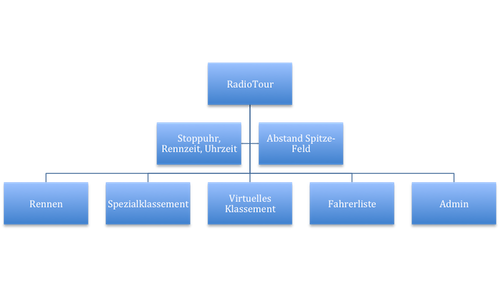
\includegraphics{05technischerbericht/images/struktur.png}
\end{figure} 


\section{Technologien}
\subsection{Android}
Die native Programmiersprache für das Android Betriebssystem ist Java. Die Programmierung in Java bringt den Vorteil, dass auf die gesamte \gls{api} von Android zugegriffen werden kann. Weiter sind die Geräte genau dafür ausgelegt und die optimale Performance kann erreicht werden. Sämtliche Komponenten dieser Arbeit sind in Java geschrieben. Für die Persistierung der Daten auf dem Tablet wird eine \gls{sqlite} Datenbank verwendet.

\subsection{Externe Libraries}
Android beinhaltet bereits ein umfangreiches Framework zur Entwicklung. Einzig beim \gls{orm}, also beim Abbilden von Objektdaten in der Datenbank kommt eine externe Library zum Einsatz.
\\
\textit{ORMLite} \footnote{ORMLite, \url{http://ormlite.com/}, Aufgerufen am 23.05.2012} ist eine OpenSource Java Library, welche auch für Android eine optimale Lösung bietet. Die zu verwendenden Felder einer Klasse können mit Java Annotationen versehen werden, daraus versucht ORMLite dann die Datenbank zu beschreiben. In der RadioTour Anwendung konnten alle Felder abgebildet werden.


\subsection{Entwicklungsumgebung}
Die von Android empfohlene Entwicklungsumgebung ist Eclipse\footnote{Eclipse, \url{http://eclipse.org/}} mit einem Plugin zur Entwicklung von Android Applikationen. Auf der Entwicklerseite von Android steht dazu folgendes:
\begin{quote}
\grqq Android Development Tools (ADT) is a plugin for the Eclipse IDE that is designed to give you a powerful, integrated environment in which to build Android applications.\grqq
\footnote{Android Plugin für Eclipse, \url{http://developer.android.com/sdk/eclipse-adt.html}}
\end{quote}
Eclipse ist eine weit verbreitete \gls{ide} und wird aktiv weiter entwickelt. Mit dem Plugin zusammen bilden Sie eine solide Grundlage für dieses Projekt.
\\
Damit die Android Applikation direkt auf dem Computer getestet werden kann, stellt Google ein Emulator zur Verfügung. Der Emulator ist allerdings auch als solcher zu betrachten da die Bedienung nicht vergleichbar ist mit einem richtigen Tablet.

\subsection{Android Version}
Eine Anwendung wird für eine spezifische Android Version entwickelt und getestet, somit kann garantiert werden, dass das Verhalten der Anwendung  immer gleich ist. In dieser Arbeit ist dies die Version 3.1 mit dem Versionsnamen \textit{Honeycomb}.\footnote{\url{Android Version Honeycomb, http://de.wikipedia.org/wiki/Android_(Betriebssystem)\#Versionsverlauf}}.
\\
Die Entwicklung auf einer Version schliesst jedoch nicht aus, dass die Anwendung in neueren Versionen nicht mehr lauffähig ist. Auch \textit{RadioTour} kann für zukünftige Versionen weiterentwickelt und verwendet werden.

\section{Mitbewerberanalyse}
Die Art der Applikation ist sehr spezifisch und kann nicht direkt auf andere Sportereignisse angewendet werden. Deshalb beinhaltet die Analyse von Mitbewerbern nur die grossen europäischen Radrennen. Wie bei der Tour de Suisse ist auch in Frankreich an der \textit{Tour de France}\footnote{Tour de France, \url{http://www.letour.fr/}} ein RadioTour Speaker mit dabei. Darüber wie die Aufzeichnungen in Frankreich im genauen stattfinden kann aber nur spekuliert werden da die Informationen nicht öffentlich zugänglich sind.
\\
In Italien findet zum Zeitpunkt dieser Arbeit der \textit{Giro d'Italia}\footnote{Giro d'Italia, \url{http://www.gazzetta.it/Speciali/Giroditalia/2012/}} statt. Bei diesem Radrennen ist es möglich aus den Informationen, welche auf der Webseite verfügbar sind, zu schliessen, dass ein ähnliches System verwendet wird. Während dem Rennen ist es möglich die aktuelle Rennsituation zu betrachten.

\begin{figure}[h!]
\caption{Rennsituation am Giro d'Italia}
\label{fig:giro}
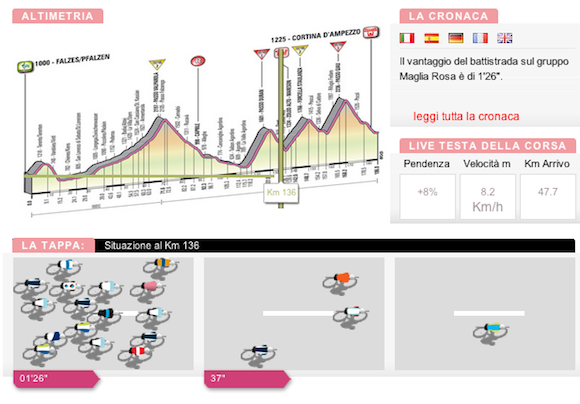
\includegraphics[scale=0.7]{05technischerbericht/images/giro.png}
\end{figure} 

In der Abbildung \ref{fig:giro} ist der Live Abschnitt der offiziellen Webseite zu sehen. Im oberen Teil wird der Standort in der aktuelle Etappe eingeblendet. Weiter unten ist die Situation an der Spitze abgebildet. Die Fahrer sind nach Rückstand gruppiert.
\\
Da jedoch nicht zu erkennen ist, wie die Informationen im Feld erfasst werden muss die Mitbewerberanalyse an dieser Stelle abgeschlossen werden.

\chapter{Architektur}
Im folgenden Abschnitt wird die Architektur der Applikation diskutiert. Die Architektur ist so gewählt, dass die einzelnen funktionalen Komponenten zueinander eine tiefe Abhängigkeit aufweisen.

\section{Domainmodel}
Die Domainlogik beinhaltet die Kernelemente der Applikation. Einerseits sind dies die Rennfahrer, welche Informationen über sich festhalten andererseits die Etappe mit den Informationen zur Strecke. Während dem Rennen werden die Fahrer in Gruppen unterteilt. Auch diese Gruppen sind in der Domain abgebildet. Das Klassendiagramm des Domain Package zeigt die wesentlichen Elemente.

\begin{figure}[h!]
\caption{Die Domainklassen in der Abhängigkeit}
\label{fig:domain}
\centering
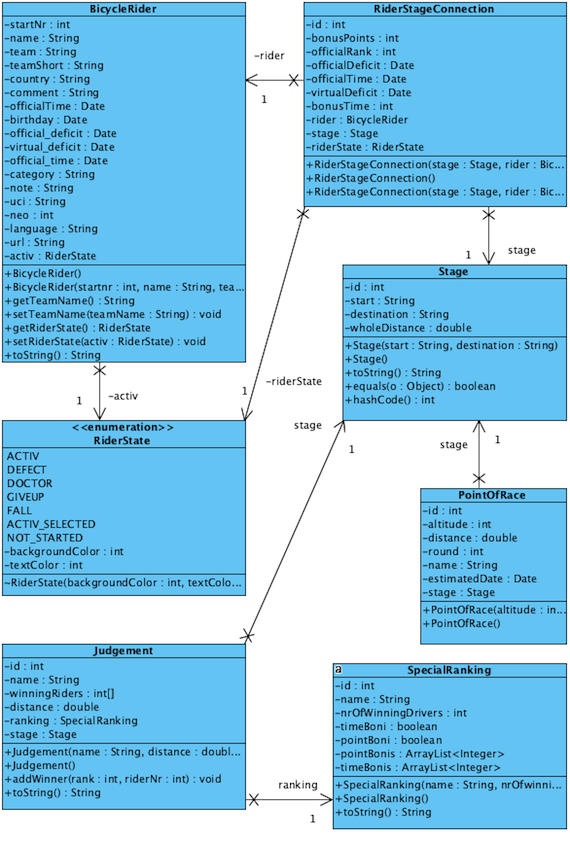
\includegraphics{05technischerbericht/images/domain.png}
\end{figure} 


\textit{BicycleRider} speichert die Angaben zu einem Fahrer und beinhaltet keine eigene Logik. Ein Fahrer hat immer genau ein \textit{RiderState}. Dies ist ein Java \gls{enum} und zeigt den Status des Fahrer an. Nach dem Import der Fahrerliste werden alle Fahrer auf \textit{activ} gesetzt.

In \textit{Stage} ist die Etappe definiert. Jede Etappe hat eine Marschtabelle in Form von mehreren \textit{PointOfRace} Objekten. Diese Objekte werden durch Import der Marschtabelle erstellt.
Da pro Etappe jeder \textit{BicycleRider} einen anderen \textit{RiderState} haben kann, gibt es die Verbindungsklasse \textit{RiderStageConnection}. In dieser Klasse ist jeweils die Etappe mit dem Fahrer verknüpft. Dies ermöglicht es den Rückstand eines Fahrers in mehreren Etappen zu verfolgen.
Ein \textit{Judgement}, also eine Wertung, gehört immer zu einer Etappe. Diese Wertungen sind definiert durch ein \textit{SpecialRanking}, welche Punkte- und Zeitboni beinhalten können.


\chapter{Realisierung}
Lorem ipsum dolor sit amet, consetetur sadipscing elitr, sed diam nonumy eirmod tempor invidunt ut labore et dolore magna aliquyam erat, sed diam voluptua. At vero eos et accusam et justo duo dolores et ea rebum. Stet clita kasd gubergren, no sea takimata sanctus est Lorem ipsum dolor sit amet. Lorem ipsum dolor sit amet, consetetur sadipscing elitr, sed diam nonumy eirmod tempor invidunt ut labore et dolore magna aliquyam erat, sed diam voluptua. At vero eos et accusam et justo duo dolores et ea rebum. Stet clita kasd gubergren, no sea takimata sanctus est Lorem ipsum dolor sit amet.

\chapter{Testing}
Lorem ipsum dolor sit amet, consetetur sadipscing elitr, sed diam nonumy eirmod tempor invidunt ut labore et dolore magna aliquyam erat, sed diam voluptua. At vero eos et accusam et justo duo dolores et ea rebum. Stet clita kasd gubergren, no sea takimata sanctus est Lorem ipsum dolor sit amet. Lorem ipsum dolor sit amet, consetetur sadipscing elitr, sed diam nonumy eirmod tempor invidunt ut labore et dolore magna aliquyam erat, sed diam voluptua. At vero eos et accusam et justo duo dolores et ea rebum. Stet clita kasd gubergren, no sea takimata sanctus est Lorem ipsum dolor sit amet.

\chapter{Ergebnisse und Schlussfolgerungen}
Lorem ipsum dolor sit amet, consetetur sadipscing elitr, sed diam nonumy eirmod tempor invidunt ut labore et dolore magna aliquyam erat, sed diam voluptua. At vero eos et accusam et justo duo dolores et ea rebum. Stet clita kasd gubergren, no sea takimata sanctus est Lorem ipsum dolor sit amet. Lorem ipsum dolor sit amet, consetetur sadipscing elitr, sed diam nonumy eirmod tempor invidunt ut labore et dolore magna aliquyam erat, sed diam voluptua. At vero eos et accusam et justo duo dolores et ea rebum. Stet clita kasd gubergren, no sea takimata sanctus est Lorem ipsum dolor sit amet.

\chapter{Verzeichnisse und Referenzen}

\section{Literaturverzeichnis}


\section{Tabellenverzeichnis}


\section{Abbildungsverzeichnis}
\listoffigures


\printglossary[style=altlist,title=Glossar]


\nocite{*}
\bibliographystyle {unsrt}
\bibliography{06verzeichnisse/02literaturverzeichnis}

\part{Anhang}

\section{BigPicture}
\label{fig:bigpicture}
Das Aufgabenumfeld in einem BigPicture zusammengefasst.
\begin{figure}
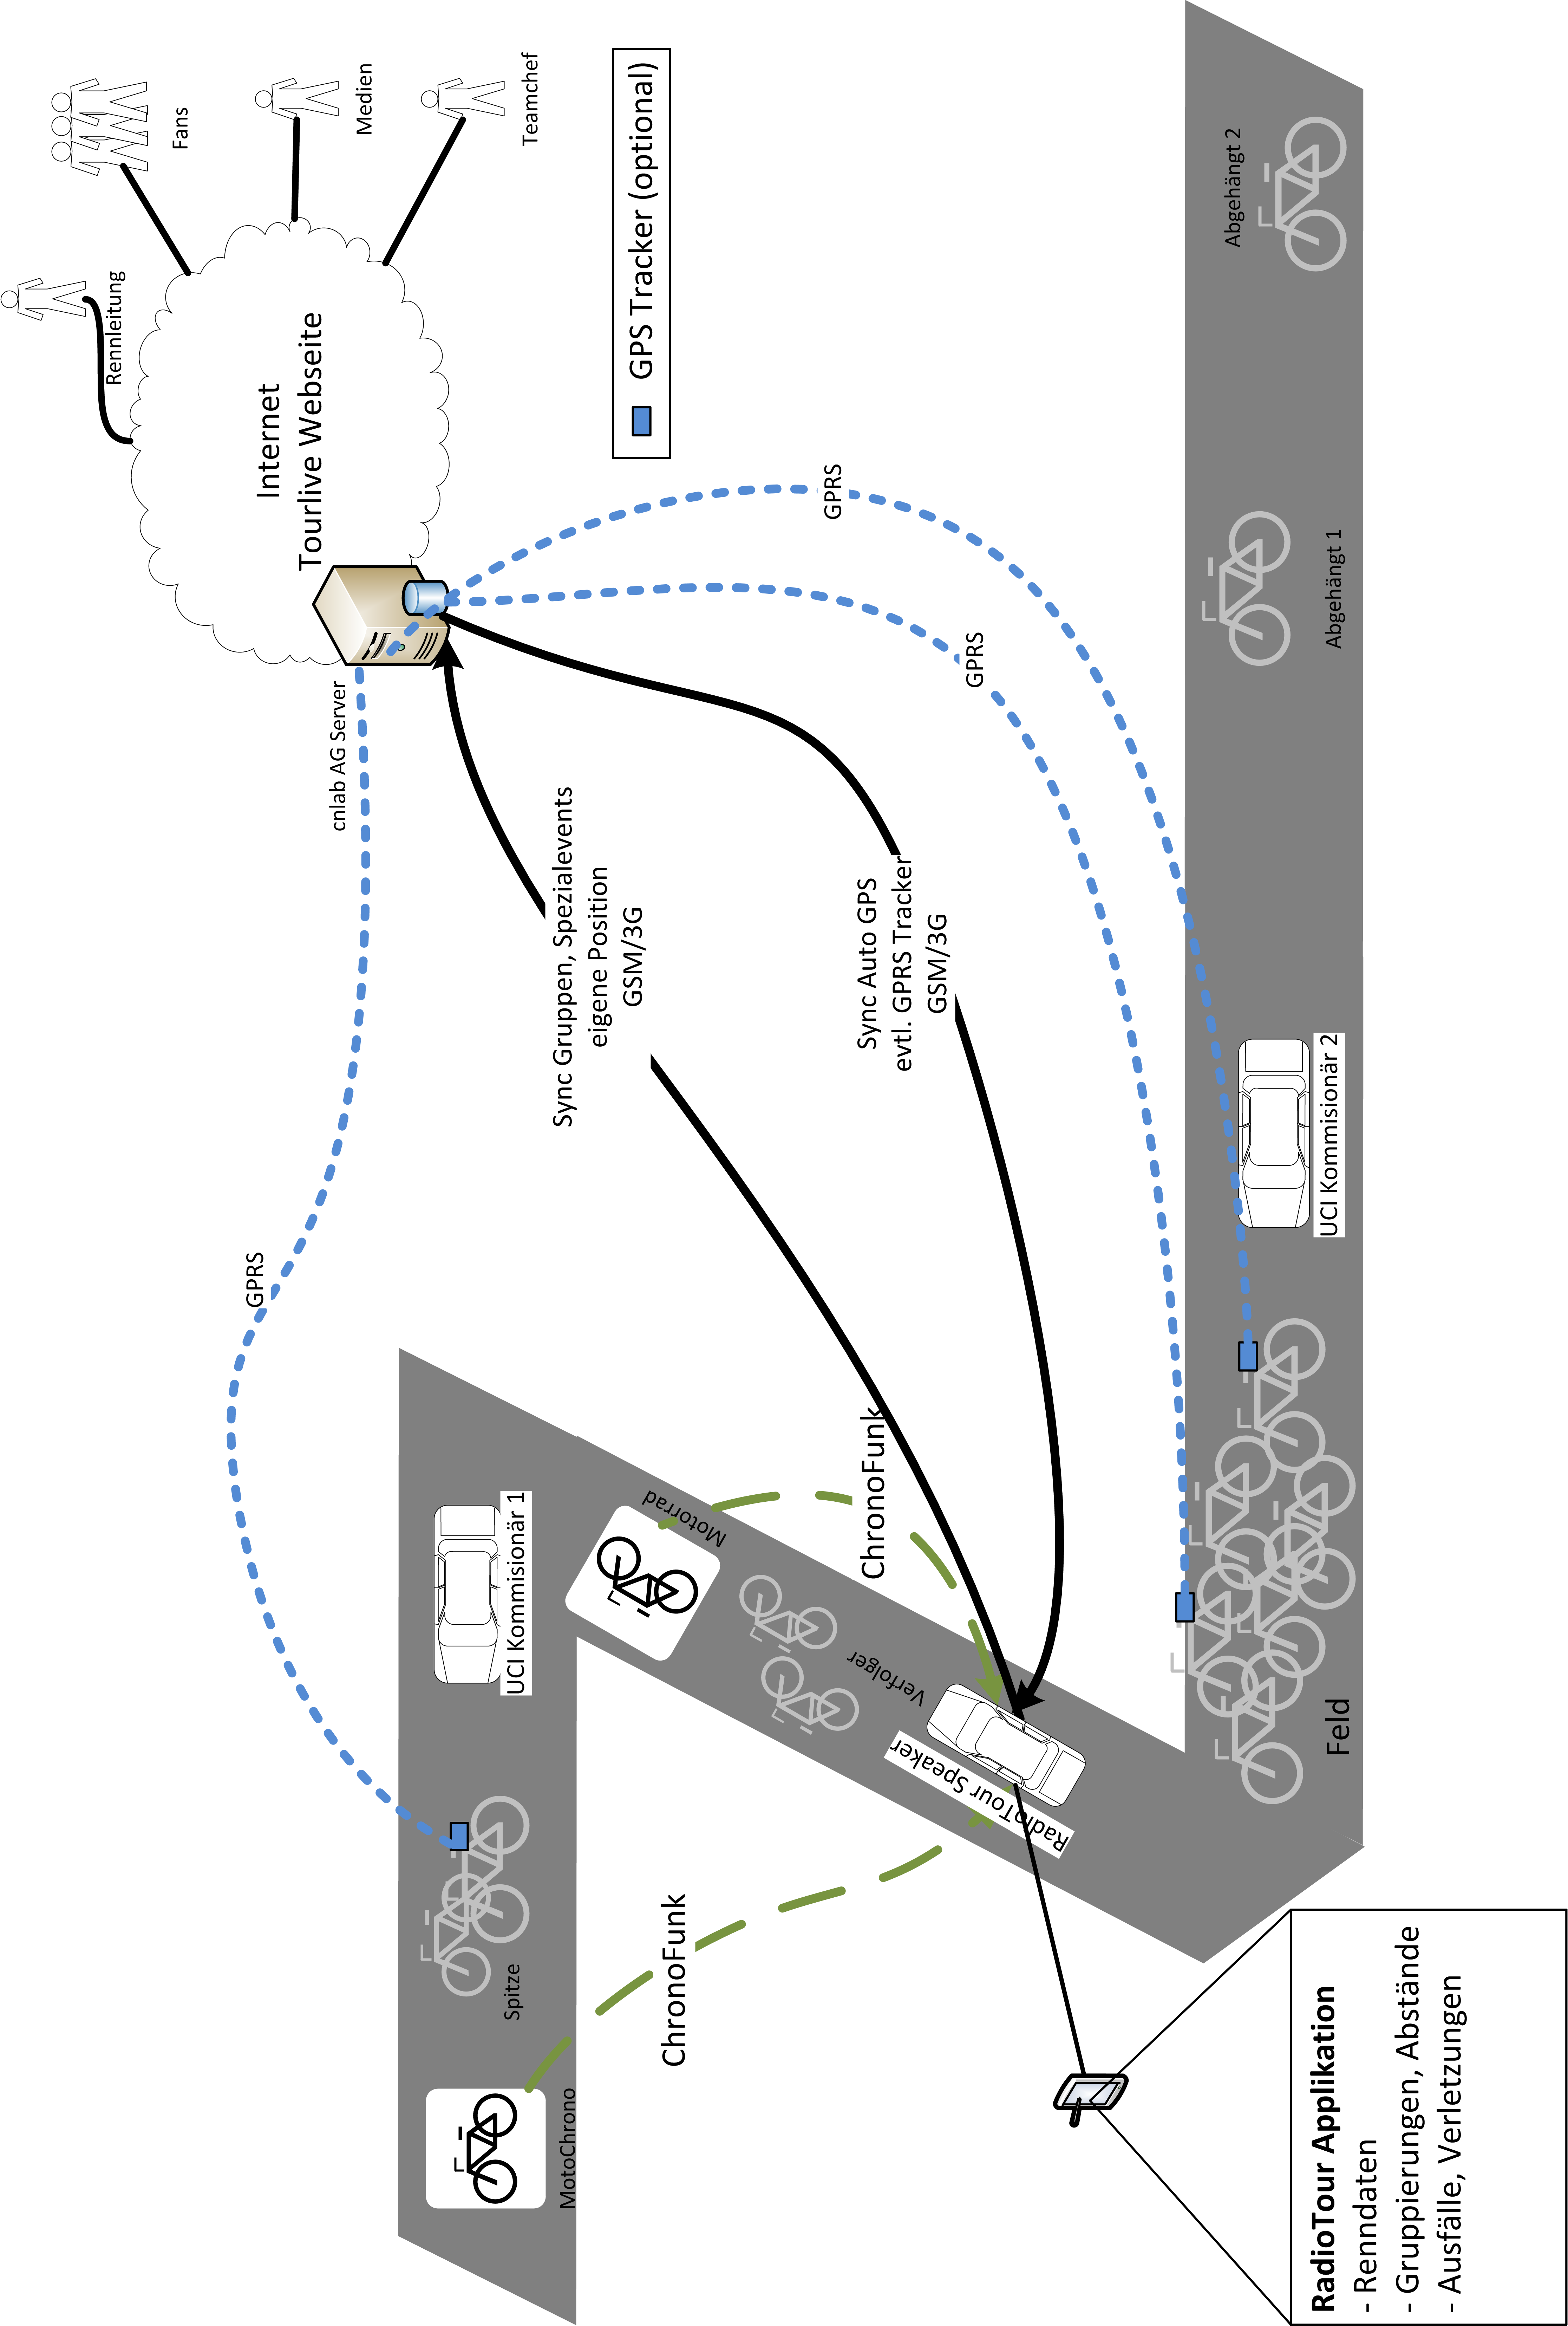
\includegraphics[scale=0.8]{07anhang/images/bigpicture.png}
\caption{Das BigPicture in voller Grösse}
\end{figure}

\section{Projektmanagement}

\section{Software Dokumente}

\section{Kriterienkatalog}
\label{ref_kriterien}
Hier sind die Kriterien

\section{Kaufempfehlung}
\label{ref_kaufempfehlung}

\section{UseCases der bisherigen Applikation}
\label{ref:usecases}
Im unten stehenden UseCase Diagramm (Abbildung \ref{fig:usecasediagram}) sind die primären UseCases aufgeführt. Nur der RadioTour Speaker erfasst Daten in dieser Applikation und ist daher der einzige Aktor. Das System wird durch die RadioTour Applikation abgebildet. Zur besseren Darstellung wurden einzelne UseCases vereinfacht oder zusammen gefasst.
\begin{figure}[h1]
  \caption{UseCase Diagramm}
  \label{fig:usecasediagram}
  \begin{center}
    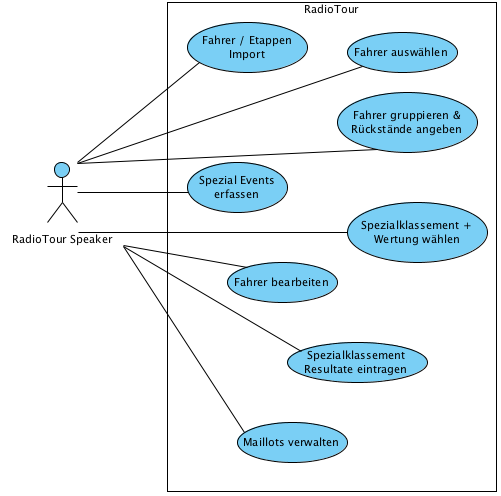
\includegraphics[scale=0.6]{05bericht/images/usecasediagram.png}
  \end{center}
\end{figure}

\begin{itemize}
\item \textbf{Fahrer auswählen}\\
Dem RadioTour Speaker muss es möglich sein, einen oder mehrere Fahrer schnell auszuwählen. Die Fahrer werden im Auswahldialog bevorzugt durch ihre Startnummern dargestellt. An der Tour de Suisse besteht ein Team – nach Aussage von P. Heinzmann – aus 8 Fahrern. Um eine möglichst gute Übersicht zu gewährleisten werden die Fahrer jeweils Zeilenweise in deren Teams gruppiert. Ausgewählte Fahrer werden farblich hervorgehoben. Die Nummern der Fahrer, welche bereits Gruppen zugewiesen wurden, werden in Klammern dargestellt. Die Nummern ausgeschiedener Fahrer werden gestrichen dargestellt.

\begin{figure}[h!]
  \caption{Die Fahrerauswahlliste zur Gruppierung in der bisherigen Web Applikation}
  \begin{center}
    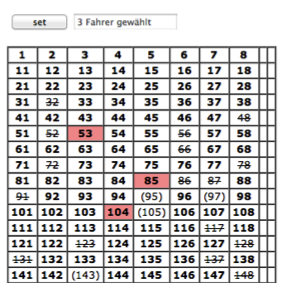
\includegraphics{05bericht/images/uc01_fahrerliste.png}
  \end{center}
\end{figure}

\item \textbf{Fahrer gruppieren}\\
Dem RadioTour Speaker muss es möglich sein, die ausgewählten Fahrer in Gruppen zu organisieren. So kann er die ihm gemeldeten Rennsituationen mit Ausreissern, Verfolgern, Feld und abgehängten darstellen.

\begin{figure}[H]
  \caption{Gruppierung in der bisherigen Web Applikation}
  \begin{center}
    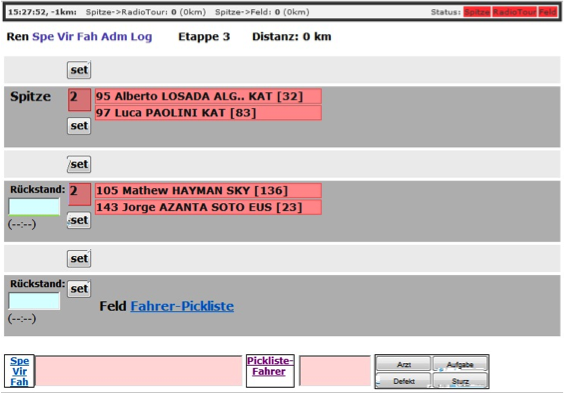
\includegraphics{05bericht/images/uc02_gruppen.png}
  \end{center}
\end{figure}

\item \textbf{Rückstände angeben}\\
Dem RadioTour Speaker muss es möglich sein, für die Gruppen (siehe oben) ihre jeweiligen Zeitabstände relativ zur Spitze einzugeben. Falls vorhanden, sollen auch die mit dem TourLive GPS-System erfassten Zeitabstände Spitze-Feld eingeblendet werden.

\item \textbf{Spezial Events erfassen}\\
Dem RadioTour Speaker muss es möglich sein, für ausgewählte Fahrer Spezialereignisse festzulegen. Dies sind beispielsweise Arztbesuch, Aufgabe, Defekt oder einen Sturz.
\begin{figure}[H]
  \caption{Die Spezialklassemente und Wertungen in der bisherigen Web Applikation}
  \begin{center}
    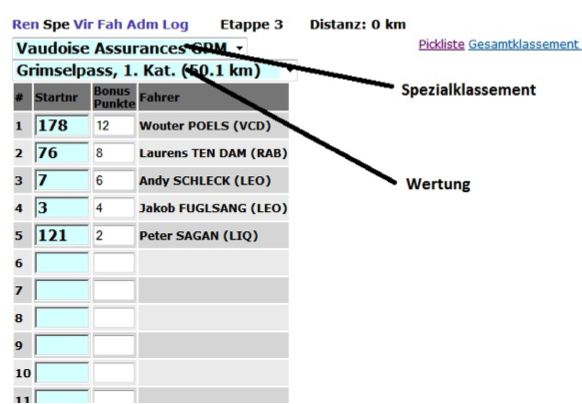
\includegraphics{05bericht/images/uc03_spezial.png}
  \end{center}
\end{figure}


\item \textbf{Spezialklassement und Wertung wählen}\\
Bei Mehretappenrennen werden typisch neben dem Gesamtklassement (schnellster Fahrer) mehrere Spezialklassemente (z.B. Bergpreis-, Sprintwertung, Punkteklassement) gewertet. Innerhalb der Etappen gibt es jeweils mehrere Stellen (Wertungen), an denen für die Spezialklassemente Punkte vergeben werden. Dem RadioTour Speaker muss es möglich sein, die gewünschte Wertung zu einem der vorher erfassten Spezialklassemente auszuwählen.

\item \textbf{Spezialklassement Resultate eintragen}\\
Dem RadioTour Speaker muss es möglich sein, für eine Wertung welche er ausgewählt hat (siehe UC oben), die Ränge zur Wertung mit Fahrernummern zu verbinden, wodurch das Klassement generiert wird.

\item \textbf{Klassement anzeigen}\\
Das durch die eingetragene Wertung erstellte Klassement muss vom RadioTour Speaker abgerufen werden können. Dort sollen alle Fahrer angezeigt werden, welche einen Punkterang in diesem Spezialklassement erreichten.

\item \textbf{Virtuelles Klassement}\\
Dem RadioTour Speaker muss es möglich sein, ein aktuelles Klassement der Tour abzurufen und dieses nach bestimmten Kriterien zu sortieren. Die zurzeit möglichen Sortierkriterien sind:
\begin{itemize}
\item[-]Gruppen (zur Zeit des Aufrufs, nicht offiziell)
\item[-]Virtueller Rückstand (zur Zeit des Aufrufs, nicht offiziell)
\item[-]Zeitboni (zur Zeit des Aufrufs, nicht offiziell)
\item[-]Offizielle Zeit (zum Etappenende des Vortages, offiziell)
\item[-]Offizieller Rückstand (zum Etappenende des Vortages, offiziell)
\end{itemize}

\begin{figure}[h!]
  \caption{Virtuelles Klassement in der bisherigen Applikation}

  \begin{center}
    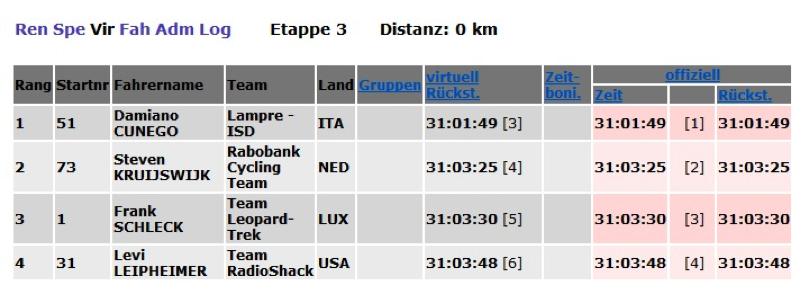
\includegraphics{05bericht/images/uc05_virtuell.png}
  \end{center}
\end{figure}

\item \textbf{Fahrerliste anschauen}\\
Dem RadioTour Speaker muss es möglich sein, die aktuelle Fahrerliste anzuschauen. Die Fahrerliste ist nach Startnummer aufsteigend sortiert. (Die Startnummern werden in Mehretappenrennen so vergeben, dass die Fahrer eines Teams aufeinanderfolgende Startnummern erhalten.)

\begin{figure}[h!]
  \caption{Die Fahrerliste mit den Informationen zum Status der Fahrer}
  \begin{center}
    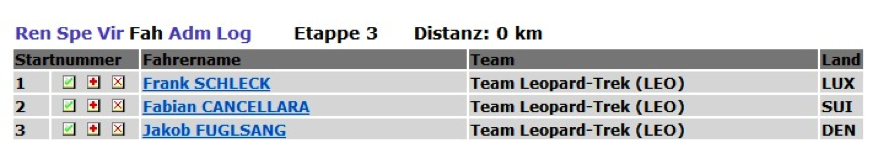
\includegraphics{05bericht/images/uc06_fahrerliste.png}
  \end{center}
\end{figure}

\item \textbf{Fahrer de- bzw. aktivieren}\\
Dem RadioTour Speaker muss es möglich sein, einzelne Fahrer zu deaktivieren bzw. wieder zu aktivieren. Der Grund der Deaktivierung soll auch später noch nachvollziehbar sein. Es soll möglich sein, den Grund für die Deaktivierung anzugeben (z.B. ausgeschieden, nicht gestartet, andere). 
Eine so vorgenommene Deaktivierung eines Fahrers muss durch den RadioTour Speaker Rückgängig gemacht werden können.

\item \textbf{Fahrerdetails bearbeiten}\\
Dem RadioTour Speaker muss es möglich sein, einen Fahrer aus der Fahrerliste auszuwählen um seine Details anzuschauen und auch zu bearbeiten. 

\item \textbf{Statistik}\\
Dem RadioTour Speaker muss es möglich sein, in seinem Admin-Bereich eine kurze und prägnante textbasierte Statistik zu erhalten, bei welcher er auf einen Blick sieht wie viele Fahrer in der Datenbank sind und welche davon aktiv sind. Darüber hinaus die Anzahl Gruppen, Spezialklassemente, Wertungen und Vergebene Punkte.

\item \textbf{Import Fahrerliste}\\
Nach jedem Renntag ( = Etappe), wird in die RadioTour Applikation eine neue Fahrerliste mit den aktuellen offiziellen Zeiten importiert. Die Herausforderung besteht darin, dass das Format dieser Fahrerlisten im vornherein nicht bekannt ist. Deshalb muss es dem RadioTour Speaker möglich sein, den Importmodus noch dynamisch anzupassen. Derzeit sind für den Import der Daten verschiedene Importverfahren implementiert wie im Screenshot ersichtlich ist.

\item \textbf{Import Spezialklassemente}\\
Dem RadioTour Speaker muss es möglich sein, Spezialklassemente zu importieren. Diese Importe werden vor der Tour de Suisse getätigt weshalb ein dynamischer Import hier nicht zwingend notwendig ist.

\item \textbf{Speicherung Maillots}\\
Dem RadioTour Speaker muss es möglich sein, die Belegung der 4 verschiedenen Maillots anzugeben und zu sichern. Folgende Maillots gibt es:

\begin{center}
  \begin{tabular}{ l | l  }
    \hline
    Name & Farbe \\ \hline
    \hline
    Bergpreis & Rot-Weiss \\ \hline
    Gesamtklassement & Gelb \\ \hline
    Neo-Profi & Weiss \\ \hline
    Punkte & Grün\\

    \hline
  \end{tabular}
\end{center}


\item \textbf{Daten exportieren}\\
Dem RadioTour Speaker muss es möglich sein, die Spezialklassemente, Wertungen, Fahrer nicht nur zu erfassen, importieren und bearbeiten, sondern auch als *.csv zu exportieren. Dabei werden einfach alle mit dem gewünschten Export assoziierten Infos in das exportierte *.csv geschrieben.

\end{itemize}




\end{document}	
